
Beyond tools like Simulink, the modeling community has pursued a number of approaches that bring model-driven development toolchains to embedded system development. For example, SysWeaver \cite{sysweaver:niz} includes a modeling tool, import capability for Simulink, code generation, and support for distributed platforms; but does not use the time-triggered model of computation  and thus lacks off-line scheduling capability.  Other tools generally do not include hardware platform modeling and analysis.

%The DECOS toolchain \cite{decos07} combines a number of existing tools (e.g. the TTech tools, SCADE from Esterel Technologies, and others) but the hardware platform modeling and analysis aspects are not covered. 

\begin{figure}[ht]
\centering
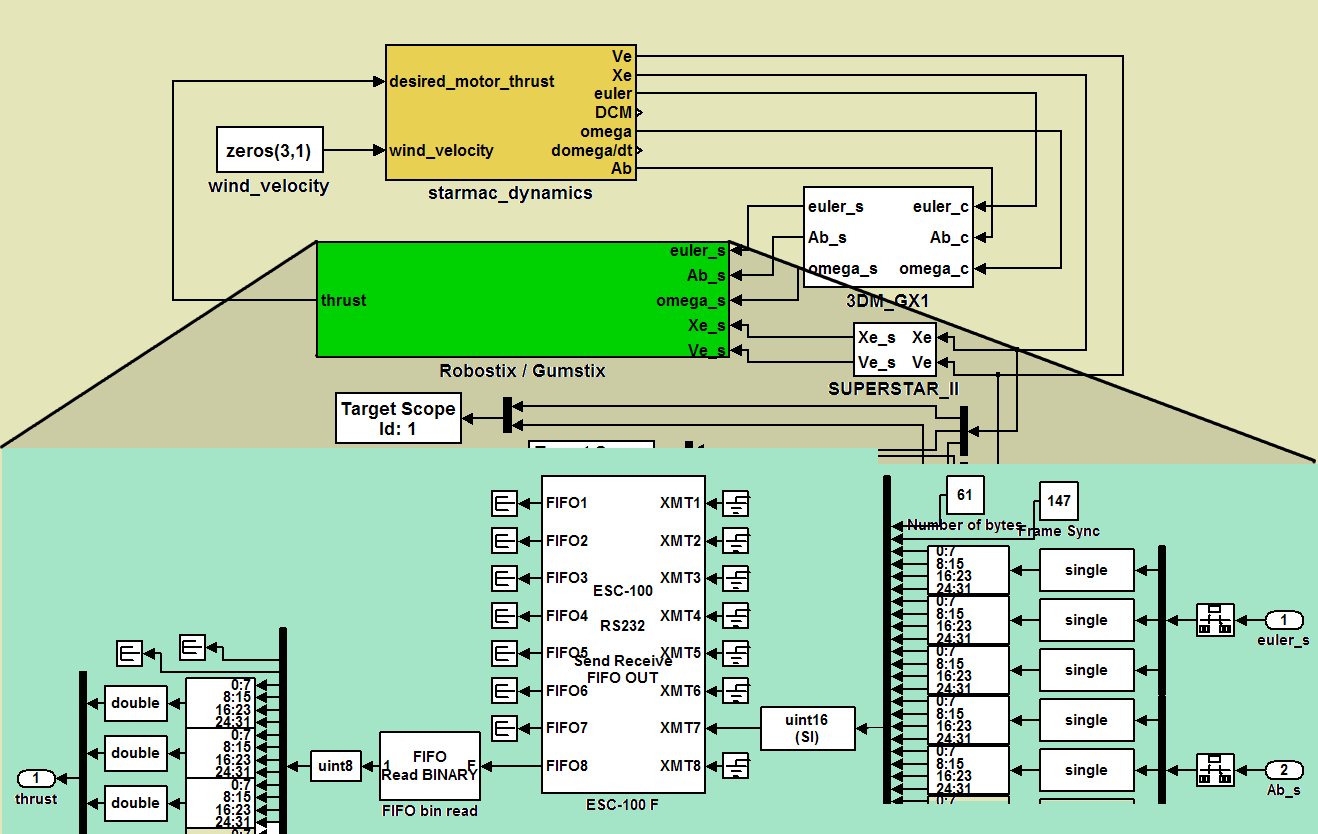
\includegraphics[width=\columnwidth]{figures/xpc_model.png}
    \caption{Plant simulation model for Mathworks' xPC Target(R)}
    \label{fig:xpc_sim}
\end{figure}

Similar goals, concepts, tools, and techniques are also found in large standardization efforts and research projects for real-time embedded systems development.  The UML profile for Modeling and Analysis of Real-Time and Embedded systems (MARTE)\cite{marte} provides software modeling tools with a framework for embedded control systems modeling and design.  The Architecture and Analysis Design language (AADL)\cite{AADL} is a textual specification language with similar aims. Projects based on these tools include modeling\cite{Topcased}, schedulability analysis\cite{cheddar}, and verification\cite{aadl_bip}.  Our effort differs in the fundamental approach -- we aim to build up a tool chain and modeling language from the ground up to experiment with design decoupling techniques, rapid integration of heterogeneous tools, and formal semantics.  The language is deliberately kept simple, containing only what we actually use.  Due to its experimental nature some parts of the language and tool infrastructure change very frequently (in contrast with standardized languages and tools).  As it expands we will seek a larger user base and possibly integration with existing tools.

